\documentclass{scrreprt}

\usepackage{libertine}
\usepackage{graphicx}
\usepackage[table,xcdraw]{xcolor} %color in tables
\usepackage{hyperref}
\usepackage{array, tabularx, caption, boldline}
\usepackage{cellspace}
\usepackage{pdfpages} 
\setlength\cellspacetoplimit{4pt}
\setlength\cellspacebottomlimit{4pt}
\usepackage{tikz}
\newcommand*\circled[1]{\tikz[baseline=(char.base)]{
		\node[shape=circle,draw,inner sep=2pt] (char) {#1};}}

\RedeclareSectionCommand[
  beforeskip=-.5\baselineskip,
  afterskip=.25\baselineskip]{subsubsection}
\RedeclareSectionCommand[
  beforeskip=-.5\baselineskip,
  afterskip=-0.5em]{paragraph}
\RedeclareSectionCommand[
  beforeskip=-.2\baselineskip,
  afterskip=-0.5em]{subparagraph}

\subject{EP Secure Cloud Energy Monitoring Platform WS 2018/19}
\title{Design}
\subtitle{Scrum Master and Product Owner: Martin Binder}
\author{Martin Binder\\Korbinian Simonis\\Benedikt Holler\\Andreas M\"uller\\Simon Sch\"onberger}
\date{As of \today}
\dedication{
  {\titlefont \LARGE Hello there!}\\
  We're Team Hams and we're doing our very best to deliver only the finest software.\\~\\
  
\includegraphics{team-normal.jpeg}
}

\begin{document}
\maketitle
\tableofcontents

\chapter{Use Case}
Author:  Andreas Müller |
Reviewer: Martin Binder\\ \\

\paragraph{User Specification.}
Three types of users have access to the EMS.
All have different rights, to create a structured work environment.
\\ 

\subparagraph{User:}
Common user, can only access the dashboardConfiguration and his profile.

\subparagraph{Privileged User:}
Has rights form user and has access to alert notifications.

\subparagraph{Administrator:}
Has privileged user rights and has access to user management and node management.



\section{Use Case}
%this is our template for the use cases.
%linebreaks are performed automatically if you reached the max width of a cell.
%if you need to force a linebreak within a cell use the \newline command.
Prerequisites to use the HAMer Tool and not explicitly mentioned in every Use Case: \\
- Access to the Intranet on which HAMer is deployed.\\
- A compatible Browser (i.e. Firefox or Chrome). \\
- A user account (provided by the administrator of the tool). \\
- The Frontend is up and reachable.
- The Backend is up and reachable. \\
 Except for UC00: \\
- User performs a correct login.
\\
\\ \\
\begin{tabularx}{12cm}{l|X}
	ID & UC01  \\
	\hline
	Label & 
	A User logs in on the EMS website. \\
	\hline
	Actor            & User    \\
	\hline
	Description            &  	1. User enters their user name. 2. User enters their password. 3. User clicks on "Login" 4. System authorizes User to access the EMS \\
	\hline
	Precondition           &   User has an valid account.\\ 
	\hline
	Postcondition     & User is logged into the system and accesses the content. \\
	\hline
	Exceptional Cases & 1. User has no account. 2. User enters wrong password. 3. User enters wrong user name. 
	4. System can't process the request.
	
\end{tabularx}
\\
\\ \\
\begin{tabularx}{12cm}{l|X}
	ID & UC02  \\
	\hline
	Label & 
	A User logs out. \\
	\hline
	Actor            & User   \\
	\hline
	Description            &  	1. User clicks log out. 2. System destroys user session.  \\
	\hline
	Precondition           &   User is logged in.\\ 
	\hline
	Postcondition     & User is logged out and can't access EMS without re-authentication. User session is destroyed. \\
	\hline
	Exceptional Cases & 1. System can't process the request.
	
\end{tabularx}
\\
\\ \\ 
\begin{tabularx}{12cm}{l|X}
	ID & UC03  \\
	\hline
	Label & 
	Evaluate KPIs. \\
	\hline
	Actor            & User   \\
	\hline
	Description            &  	1. User accesses the Dashboard.	
	2. User sees Overview of energy consumption of all supervised nodes. 3. User picks a specific node. 4. User picks specific KPI. 5. User enters date and time period. 5. System provides visualized data for the entered conditions.
	\\
	\hline
	Precondition           & 1. User has a valid account. 2. User performs a successful login. 3. KPIs exist for the picked time frame.  \\
	\hline
	Postcondition     & System provides specific data on the picked KPI in a certain time frame. \\
	\hline
	Exceptional Cases & 1. KPIs don't exist. 2. System can't process the request.

\end{tabularx}
\\
\\ \\ 

\begin{tabularx}{12cm}{l|X}
	ID & UC04  \\
	\hline
	Label & 
	A User edits their profile. \\
	\hline
	Actor            & User    \\
	\hline
	Description            &  	1. User clicks on "Edit Profile" on the Navigation Bar on the left side of the screen. 2. System redirects User to the Edit Profile page. 3. User edits their profile(email, password etc.) 4. System saves changes on the Users profile.   
	\\
	\hline
	Precondition           & 1. User has a valid account. 2. User is logged in.  \\
	\hline
	Postcondition     & BE processes the changes and updates the database. \\
	\hline
	Exceptional Cases & 1. Input is invalid. 2. System can't process the request.
	
\end{tabularx}
\\
\\ \\

\begin{tabularx}{12cm}{l|X}
	ID & UC05  \\
	\hline
	Label & 
	User sets their Alert Notification. \\
	\hline
	Actor            & Privileged User  \\
	\hline
	Description            &  	1. User clicks on "Alert Notification" on the Navigation Bar on the left side of the screen. 2. System redirects User to the Alert Notifications page. 3. User creates an alert notification. 4. User assigns alert notification to nodes. 5. User clicks on "Save changes" 6. System saves changes.   
	\\
	\hline
	Precondition           & 1. User has a valid account. 2. User is logged in.   \\
	\hline
	Postcondition     &  New alert notification is in database. 2. Alert notification is assigned to nodes. \\
	\hline
	Exceptional Cases & 1. Input is invalid. 2. System can't process the request.
	
\end{tabularx}
\\
\\ \\ 

\begin{tabularx}{12cm}{l|X}
	ID & UC06  \\
	\hline
	Label & 
	An Administrator manages user account. \\
	\hline
	Actor            & Administrator   \\
	\hline
	Description            &  	1. Administrator clicks on "User Management" on the Navigation Bar on the left side of the screen. 2. System redirects Administrator to the User Management page. 3. Administrator manages user profile. 4. System saves changes on the Users profile.   
	\\
	\hline
	Precondition           & 1. Administrator has a valid account. 2. Administrator is logged in.  \\
	\hline
	Postcondition     & BE processes the changes and updates the database. \\
	\hline
	Exceptional Cases & 1. Input is invalid. 2. System can't process the request.
	
\end{tabularx}
\\
\\ \\
\begin{tabularx}{12cm}{l|X}
	ID & UC07  \\
	\hline
	Label & 
	An Administrator manages nodes. \\
	\hline
	Actor            & Administrator    \\
	\hline
	Description            &  	1. Administrator clicks on "Node Management" on the Navigation Bar on the left side of the screen. 2. System redirects Administrator to the node management page. 3. Administrator manages nodes. 4. Administrator clicks on "Save changes". 5. System saves changes.  
	\\
	\hline
	Precondition           & 1.Administrator has a valid account. 2. Administrator is logged in.  \\
	\hline
	Postcondition     &  BE processes the changes and updates the database.\\
	\hline
	Exceptional Cases & 1. Input is invalid. 2. System can't process the request.
\end{tabularx}
\\
\\ \\
\begin{tabularx}{12cm}{l|X}
	ID & UC08  \\
	\hline
	Label & 
	Administrator installs MCs. \\
	\hline
	Actor            & Administrator    \\
	\hline
	Description            &  	1. Administrator connects via ssh to node. 2. Administrator copies MC software to node. 3. Administrator runs the installation script on the MC. 4. The script installs the MC on the node. 
	\\
	\hline
	Precondition           & 1. Administrator has access to node. 2. Administrator owns MC HAMer software.  \\
	\hline
	Postcondition     &  MC is installed on node and registered on Backend \\
	\hline
	Exceptional Cases & Node does'nt meet software requirements. 
	
\end{tabularx}
\\
\\ \\


% ----------------------------------------- %
\section{User Story}
Author: Teamwork
\subsection{INVEST Principle}
The User stories follow the \textbf{INVEST} principle. To count as a User Story the following requirements have to be met: 

\paragraph{I = Independent} User Stories can't be dependent on other User Stories. If that's the case the Story has to be split up, written in a more generic way or if that's not possible, dropped..
\paragraph{N = Negotiable} The term negotiable means that User Stories have to leave some room for changes if necessary.
\paragraph{V = Value} They increase the product value. 
\paragraph{E = Estimate-able} The cost of implementation is estimate-able if a User Story can't be estimated in a foreseeable way it has to be dropped.
\paragraph{S = Small} The User Stories are as small as possible and if possible split down into an atomic form.
\paragraph{T = Testable} The outcome can be tested. If the outcome is vague the User Story has to be dropped.  \\
 \subsection{Cost Estimation}
The cost estimation follows the following rule of thumb: \\
\begin{tabular}{c|c}
	Story Point Value E & Expenditure \\ 
		\hline
		0 & No 	\\
		1 & Tiny 	\\
		2 & Small	\\
		3 & Medium	\\
		5 & Large	\\
		8 & XL	\\
		13 & XXL	\\
		20 & XXXL	\\
		40 & Massive	\\
\end{tabular}
\subsection{User Stories}
Assignee and Story Point Estimation will be done in the sprint planning of phase 4. \\
For reference see US101.
	\includepdf[width=15cm, pages=-]{s02_hams_productbacklog_export.pdf}
	\label{userstory}

\chapter{System Architecture}
% ================================================================ %


\section{Frontend}
% ----------------------------------------- %
Author: Simon Sch\"onberer | Reviewer: Martin Binder
\subsection{Technologies}
\paragraph{nuxt.js.} Nuxt is a flexible frontend framework which supports building flexible
reactive Single Page Applications on top of \emph{vue.js}. With nuxt, there are coming a few
libraries from the nuxt-ecosystem by default: \emph{vue-router} (SPA routing), \emph{vuex}
(state management) and \emph{vuetify} (material design components).

\subsection{Architecture}
\paragraph{MVVM.} Vue.js provides the architectural core of the Frontend. It is a \emph{MVVM}
framework which supports building MVVM-based SPAs. Therefore our Frontend application will be
heavily based on the MVVM pattern.
\\ \\ 
\begin{figure}[h]
	\centering
	\includegraphics[width=12cm]{mvvm-architecture.pdf}
	\caption{Navigation flow state chart}
	\label{MVVM}
\end{figure}
\\

On a low-level view, each component will use vue's component-based approach to develop
reusable components that consist of \emph{View} and \emph{ViewModel} each. They will be bound
to the model via a nuxt.js helper called \emph{asyncData}, but anyway, the model consists 
just of asynchronous HTTP-calls or incoming STOMP-updates (see \#STOMP API ref). Vue.js takes
care of data binding between View and ViewModel, to make them independent of each other.
Note that vue keeps things simple by reducing data binding to a lowest possible level by
default, and therefore only enables single-way-bindings by default. By using the dedicated
API functions provided, two-way-bindings can be easily accomplished and will be used in our
application wherever it adds value.

On a higher level, many components will be put together to build the application. Those components
can be roughly divided into three categories, according to the structure nuxt leverages:
\emph{Pages}, \emph{(reusable) Components} and \emph{Layouts}.
Layouts define template-like structures, where the route-dependent content can be wrapped in.
Pages will provide a logical unit of the applications interfaces, even in terms of routing.
They will represent a view or part of a view like e.g. "Dashboard".
Last but not least, Components build small, heavily reusable units which implement widely used
functions like single buttons, text inputs, etc.

\emph{Maybe merge this with "Components" and go on writing about the definitive components here.}

\subsection{Views}
Author:  Andreas M\"uller |
Reviewer: Benedikt Holler\\ \\

\begin{figure}[h]
	\centering
	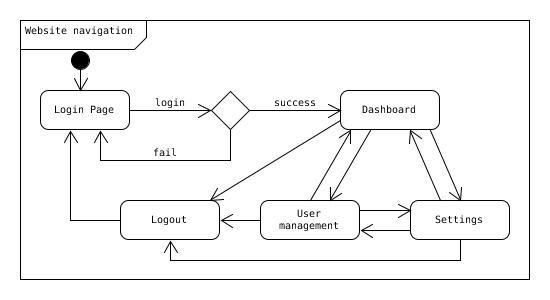
\includegraphics[width=15cm]{websiteStateChart.pdf}
	\caption{Navigation flow state chart}
	\label{navigation}
\end{figure}

\paragraph{Login.} The login view queries the user for credentials which shall be submitted
consequently. When the credentials are valid, the user will be forwarded to the dashboardConfiguration,
otherwise an error message will be added to the login view. The login view comes with the 'blank'
layout. See Figure \ref{login} for the prototype.
\begin{figure}
  \centering
  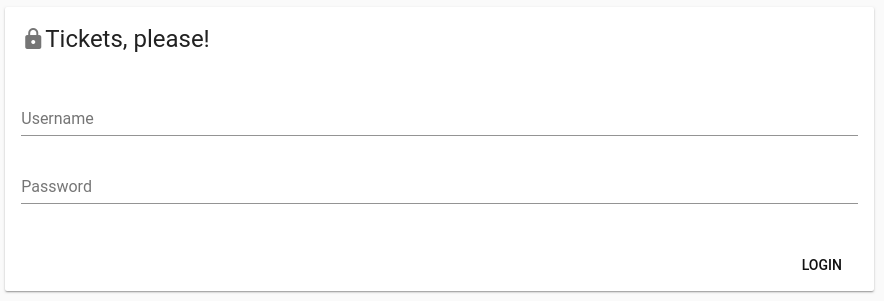
\includegraphics[width=.7\linewidth]{prototype/login}
  \caption{Prototype of the login page.}
  \label{login}
\end{figure}
%-------------------------------------------%
\paragraph{Dashboard}
After login the first page shown is the dashboardConfiguration.
The dashboardConfiguration provides graphical representation of KPIs from a selected node over a selected period.
If the dashboardConfiguration was accessed first time this session, the selected node is the first node listed, and the selected time period is the last hour.
To change the displayed node, users can select a node from a drop down list.
To visualize a different time period, users can select the date via calendar and time per drop down.

\paragraph{Menu}
The menu on the left side allows easy and fast navigation between Dashboard, User Profile, Alert Notification, Node Management, User Management and the logout button.
For example, to access the User Profile page, one only needs to click on User Profile in the menu bar.
The currently selected page is highlighted so the user knows on which page he is.

\paragraph{User Profile}
Every User has access to User Profile. Here the User can change their password and e-mail address.

\paragraph{Alert Notification}
Only privileged Users can access this page. On this page the User can manage alert rules, e.g. the user can change the text/thresholds of an alert notification or change the nodes that the alert notification is assigned to.\\
To avoid false positives due to oscillation, the User is able to smooth aberrations. Therefore it shall be possible to set the acceptable number of threshold violations for a certain period of time. If this number is exceeded, an Alert Notification is sent.

\paragraph{User Management}
An Administrator can create/delete/edit other users, for instance giving an user privileged rights.
Additionally the Administrator can create user groups and assign users to the group.

\paragraph{Node Management}
Similar to User Management, only Administrators have access to this page. Administrators can change the KPI time interval of a node
and decide which user group has access to a node.

\paragraph{Logout}
After a click on logout, the user session is destroyed and the User is redirected to the login
screen. To access the EMS again, the User must re-authenticate.

\subsection{Components}
~
\begin{figure}[!h]
	\centering
	\includegraphics[width=15cm]{s02_hams_fe-components.pdf}
	\caption{Rough overview over FE component architecture.}
	\label{fecomp}
\end{figure}

\section{Backend}
% ----------------------------------------- %
Author: Simon Sch\"onberer | Reviewer: Martin Binder\\ 

The Backend is based on the good old three-tire-architecture and will make use of a few specific
design pattern where applicable.

\subsection{Structure}
\begin{figure}[h]
	\centering
	\includegraphics[width=7cm]{3tier.pdf}
	\caption{3-tier architecture with communication flow}
	\label{3tier}
\end{figure}
\paragraph{Representation Tier.} The controller-classes in this tier are responsible for the Backend's communication with the outside world. In particular the provide the APIs specified in. \\
\textbf{Used Technologies:} HTTPS, WSS, see \ref{api}.

\paragraph{Business Logic Tier.} The business logic tier provides the core functionalities of the application as it is in control of how data is processed. 

\paragraph{Persistence Tier.} The persistence tier represents the database and data access layer which can be accessed by the business logic using the API specified in \ref{api}. \\
\textbf{Used Technologies:} Spring Data JPA

\subsection{API}
\label{api}
Author: Martin Binder | Review: Benedikt Holler
\subsubsection{FE -- BE: User Management HTTPS}
\begin{tabularx}{12cm}{l|l}
	Path & \url{/users} \\\hline
	Request Method & POST \\\hline
	Description & Create a new User.
\end{tabularx}
\\
\\ \\
\begin{tabularx}{12cm}{l|l}
	Path & \url{/users} \\\hline
	Request Method & GET \\\hline
	Description & Get all User.
\end{tabularx}
\\
\\ \\
\begin{tabularx}{12cm}{l|l}
	Path & \url{/users/:id} \\\hline
	Request Method & GET \\\hline
	Description & Get a specific User.
\end{tabularx}
\\
\\ \\
\begin{tabularx}{12cm}{l|l}
	Path & \url{/users/:id} \\\hline
	Request Method & PUT  \\\hline
	Description & Edit an existing User.
\end{tabularx}
\\
\\ \\
\begin{tabularx}{12cm}{l|l}
	Path & \url{/users/:id} \\\hline
	Request Method & DELETE \\\hline
	Description & Delete a specific User
\end{tabularx}
\\
\\ \\
\subsubsection{FE -- BE: User Groups HTTPS}
\begin{tabularx}{12cm}{l|l}
	Path & \url{/usergroups} \\\hline
	Request Method & POST \\\hline
	Description & Create a new user-group.
\end{tabularx}
\\
\\ \\
\begin{tabularx}{12cm}{l|l}
	Path & \url{/usergroups} \\\hline
	Request Method & GET \\\hline
	Description & Get all user-groups.
\end{tabularx}
\\
\\ \\
\begin{tabularx}{12cm}{l|l}
	Path & \url{/usergroups/:id} \\\hline
	Request Method & GET \\\hline
	Description & Get a specific user-group.
\end{tabularx}
\\
\\ \\
\begin{tabularx}{12cm}{l|l}
	Path & \url{/usergroups/:id} \\\hline
	Request Method & PUT  \\\hline
	Description & Edit an existing user-group.
\end{tabularx}
\\
\\ \\
\begin{tabularx}{12cm}{l|l}
	Path & \url{/users/:id} \\\hline
	Request Method & DELETE \\\hline
	Description & Delete a specific user-group
\end{tabularx}
\\
\\ \\
\subsubsection{FE -- BE: Nodes HTTPS}
\begin{tabularx}{12cm}{l|l}
	Path & \url{/nodes} \\\hline
	Request Method & GET \\\hline
	Description & Get a List of Nodes.
\end{tabularx}
\\
\\ \\
\begin{tabularx}{12cm}{l|l}
	Path & \url{/nodes/:id} \\\hline
	Request Method & GET \\\hline
	Description & Get a specific Node.
\end{tabularx}
\\
\\ \\
\begin{tabularx}{12cm}{l|l}
	Path & \url{/nodes} \\\hline
	Request Method & PUT \\\hline
	Description & Update a specific Node.
\end{tabularx}
\\
\\ \\
\begin{tabularx}{12cm}{l|l}
	Path & \url{/node/:id} \\\hline
	Request Method & Delete \\\hline
	Description & Delete a specific Node.
\end{tabularx}
\\
\\ \\
\subsubsection{FE -- BE: Alert Configuration HTTPS}
\begin{tabularx}{12cm}{l|l}
	Path & \url{/alerts} \\\hline
	Request Method & POST \\\hline
	Description & Create an Alert Configuration
\end{tabularx}
\\
\\ \\
\begin{tabularx}{12cm}{l|l}
	Path & \url{/alerts} \\\hline
	Request Method & GET \\\hline
	Description & Get a List of all Alert Configurations.
\end{tabularx}
\\
\\ \\
\begin{tabularx}{12cm}{l|l}
	Path & \url{/alerts/:id} \\\hline
	Request Method & GET \\\hline
	Description & Get a specific Alert Configuration.
\end{tabularx}
\\
\\ \\
\begin{tabularx}{12cm}{l|l}
	Path & \url{/alerts} \\\hline
	Request Method & PUT \\\hline
	Description & Update an Alert Configuration.
\end{tabularx}
\\
\\ \\
\begin{tabularx}{12cm}{l|l}
	Path & \url{/alerts/:id} \\\hline
	Request Method & DELETE \\\hline
	Description & Delete a specific Alert Configuration.
\end{tabularx}
\\
\\ \\
\subsubsection{FE -- BE: Server Settings HTTPS}
\begin{tabularx}{12cm}{l|l}
	Path & \url{/settings} \\\hline
	Request Method & GET \\\hline
	Description & Get the Server Settings.
\end{tabularx}
\\
\\ \\
\begin{tabularx}{12cm}{l|l}
	Path & \url{/settings} \\\hline
	Request Method & PUT \\\hline
	Description & Update the Server Settings.
\end{tabularx}
\subsubsection{FE -- BE: STOMP OVER WSS}
\begin{tabularx}{12cm}{l|l}
	Path & \url{/topics/dashboardConfiguration} \\\hline
	Request Method & SUBSCRIBE \\\hline
	Description & FE subscribes to topic.
\end{tabularx}
\\
\\ \\
\begin{tabularx}{12cm}{l|l}
	Path & \url{/topics/dashboardConfiguration} \\\hline
	Request Method & UNSUBSCRIBE \\\hline
	Description & FE cancels the connection. 
\end{tabularx}
\\
\\ \\
\subsubsection{MC -- BE: Nodes HTTPS}
\begin{tabularx}{12cm}{l|l}
	Path & \url{/mc/register} \\\hline
	Request Method & POST \\\hline
	Description & MC registers with the BE. 
\end{tabularx}
\\
\\ \\
\subsubsection{MC -- BE: Nodes WSS}
\begin{tabularx}{12cm}{l|l}
	Path & \url{/mc/kpi/} \\\hline
	Request Method & SEND \\\hline
	Description & MC sends a set of KPIs to the BE. 
\end{tabularx}
\\
\\ \\
\section{Monitoring Client}
% ----------------------------------------- %
In this section we describe the Monitoring Client, in particular the technology used, the architecture and the communication with the BE.

\subsection{Technology}
Our MC will be written in Python, since it's a very powerful and yet easy understandable language. Python's design philosophy emphasizes code readability and simplicity, which results in a very intuitive way of programming. As Python is an extensible programing language, there a plenty of modules, providing additional functionalities to use. \\
In concrete, we decided to use \textbf{Python3}, because it is unlike Python2 under active development. This means that all recent standard library improvements, for example, are only available by default in Python 3.x. \\
In order to implement the desired functionality, a variety of standard libraries will be needed, such as \textit{sys}, \textit{os}, \textit{http}, \textit{json}, \textit{subprocess}, \textit{multiprocessing} but also some custom libraries like \textit{psutil}, which will be the core module for our KPI collecting. \\
\textbf{psutil} is a cross-platform library mainly used for monitoring, profiling, limiting resources and for managing processes. It provides information on running processes and system utilization (CPU, memory, disks, network, sensors) and implements therefore already many functionalities offered by UNIX command line tools such as netstat, ps, lsof and top. Psutil supports currently all common platforms like Linux, Windows, macOS, FreeBSD and Sun Solaris.

\subsection{Architecture}
Since we will using Python and the required functionalities are straight forward, there is no need for complicated design pattern, that is why we plan on following the \textbf{KISS-principle} (Keep it simple, stupid) for the architecture of our MC.  
But for the sake of clarity and to facilitate maintenance, we will segment our script in a main script and several modules.
\paragraph{modules}: We plan on providing for every KPI and the energy measurement an extra module, which can be imported in our main script. A Python module is a file containing definitions and statements. 
\paragraph{main}: We plan on utilizing multiprocessing to ensure maximum responsiveness to possible configuration changes, such as the sending interval of a node. In concrete we want to use a process for the KPI collecting/sending (collector) and one for the process managing (manager). In the collector, the imported energy/KPI functions are executed in a while-loop and at the end of every loop, the KPI-Package (JSON format) is send to the BE. The manager starts/stops the collector and listens to changes from the BE.

\paragraph{class diagram}:
\begin{figure}[h]
	\centering
	\includegraphics[width=15cm]{mc_class_diagram.pdf}
	\caption{Class diagram of our MC}
	\label{class_mc}
\end{figure}
\subsection{Communication}
The only communication the MC needs to provide, is to the BE.
Here we have to cover three different scenarios. \\
On the one hand the registration of a client on the backend, on the other hand the sending of KPI packages to the BE and the receiving of configuration changes from the BE.
For the registration, we will use https as shown in \textbf{MC | BE: Nodes HTTPS} in Section \ref{api}. \\
For the other two connections we will use websockets (Section \ref{websockets}). The MC subscribes to a topic on the BE and receives configuration changes over WSS (websocket secure). Since websockets provide a two-way interactive communication session, the collector can also use this connection to send the KPI packages (see Section \ref{api}, \textbf{MC | BE: Nodes WSS}).

% ================================================================ %
\chapter{Data Model}
\section{Use Case Diagram}
\begin{figure}[h!]
	\centering
	\includegraphics[scale=0.8]{usecasediagram1.pdf}
	\caption{Simplified view Use Case}
	\label{usecase1}
\end{figure}	

% ----------------------------------------- %
\section{Entity Relationship Model}
\begin{figure}[h!]
	\centering
	\includegraphics[scale=0.65, angle=270]{er.pdf}
	\label{er}
\end{figure}	

% ----------------------------------------- %
From the ER model above, we deduced the following Database Schema. \\ 
Attributes written in \textbf{bold} constitute that table's Primary Key. Attributes in \emph{italics} are Foreign Keys, and the attribute in the foreign table they reference is in brackets.\\ \\
\begin{tabularx}{12cm}{l|X}
	\hline 
\textbf{Table Name}	& \textbf{Attributes} \\ 
	\hline 
Nodes	&\textbf{ID:Long}, Send\_Interval:Long  \\ 
	\hline 
KPI\_Packages	& \textbf{Timestamp:Long}, \textbf{\emph{OriginNode:Long(Nodes.ID)}}, CpuU:Float, RamU:Float, NetT:Float, Tempts: Float, EneC:Float \\ 
	\hline 
Users	& \textbf{ID:Long}, E-Mail:String, Name:String, Password:String  \\ 
	\hline 
User\_Groups	&\textbf{ID:Long}, Name:String  \\ 
	\hline 
Alert\_Rules	&\textbf{ID:Long}, CpuTh:Float, RamTh:Float, NetTh:Float, TemTh:Float, EneTh:Float, Smoothing:Field, \emph{ConfiguredBy:Long(Users.ID)}  \\ 
	\hline 
Notifications	&\textbf{ID:Long}, Timestamp:Long, Text:String, \emph{Recipient:Long(Users.ID)} \\
\hline 
Rule\_Designations & \textbf{\emph{Rule:Long(Alert\_Rules:ID)}}, \textbf{\emph{Node:Long(Nodes.ID)}}  \\ 
	\hline 
Node\_Assignments	&\textbf{\emph{Node:Long(Nodes.ID)}}, \textbf{\emph{User\_Group:Long(User\_Groups.ID)}}  \\ 
	\hline 
Group\_Memberships	&\textbf{\emph{User:Long(Users.ID)}}, \textbf{\emph{Group:Long(User\_Groups.ID)}}  \\ 
	\hline 
\end{tabularx} 
\section{Domain Model}
% ----------------------------------------- %
In this section we provide the jpa domain class diagram. \\
In order to keep it simple and clear, the respective getter and setter methods of the individual attributes are not depicted in the diagram.
\begin{figure}[h]
	\centering
	\includegraphics[width=15cm]{s02_hams_be-domainclasses}
	\caption{Domain class diagram}
	\label{class_domain}
\end{figure}

\chapter{Control Flow}
% ================================================================ %
Author: Martin Binder | Review: 
\section{Authentication}
To provide Users with secure Authorization of their requests JSON Web Token \textbf{JWT} is used. The issue is that JWT itself does'nt provide a secure form of Authentication. This problem is solved by a small open source plug-in called security-jwt which is available under \\
\fbox{\parbox{0.93\linewidth}{https://github.com/bratkartoffel/security-jwt-examples}}

% ----------------------------------------- %
\section{STOMP over Websocket} \label{websockets}
For the connection between FE and BE and also between MC and BE we decided to use STOMP over WebSocket to enable a near real time and  pushed-by-the-server continuous connection.

\subsection{Websocket}
To satisfy the demands of the communication architecture between the FE, BE and MC, where the BE pushes updates without the FE explicit request (always when they become available), we chose WebSocket as the continuous connection to enable the desired behavior. With WebSocket data that is received by the BE (i.e. new sets of KPIs) can be pushed to the FE, thus enabling an efficient full duplex communication. In the same way, configuration changes regarding the MCs are pushed to the MCs by the BE as fast as the Backend becomes aware of them. Another major advantage is the compared small package size and low latency that WebSocket protocol provides which saves resources and leads in smoother scaling.
\subsection{Simple(Streaming) Test Oriented Messaging Protocol}
STOMP is an implementation-agnostig simple and lightweight messaging protocol. We decided
to use it in order to add stronger semantics on top of the raw WS-frames. It provides a few
operations like \texttt{CONNECT, DISCONNECT, SUBSCRIBE, UNSUBSCRIBE, SEND} and a few others
which allow clients to interact whith message brokers.
STOMP offers a simple leightweight solution to handle the communication between client and server. With the focus on messaging semantics especially the STOMP frames and the key/value pairs used in STOMP messages. Those allow an easy implementable solution to how new KPIs are sent and can easily be understood by the FE and facilitates continuous updates.
After an initial handshake, clients can subscribe themselves to certain topics and
receive data whenever the topic gets updated by the message broker. They are also able to
send messages to the message broker.

In our application, the BE will act as a message broker for FE and MCs. The FE subscribes to
a topic, to which updates to the current Dashboard get published. Each MC subscribes to
a topic, on which configuration changes will be pushed. Vice versa the MCs send messages
whith KPI updates to the BE.

% ----------------------------------------- %
\section{Alert}
Email alerts are sent using the JavaMailSender interface for which spring boot provides an auto-configuration that enables a quick and easy implementation. With some minor setting changes a Bean can be configured with an Email address that will be used to send notifications to Users in case the configured threshold for a node is exceeded. As for the development phase a Google SMTP server will be used until an usable Email address is provided by the customer.
% ----------------------------------------- %

\section{Sequence diagram}
Author:  Andreas M\"uller |
Reviewer: Simon Sch\"onberger\\ \\
% ----------------------------------------- %
The following sequence diagram describes the use-case "Login". \\
A User enter his credentials in the login page.
\\ \\
\begin{figure}[h]
	\centering
	\includegraphics[width=15cm]{sequenceLogin.pdf}
	\caption{Sequence diagram: Login}
	\label{alertSequence}
\end{figure}

\pagebreak\
\\
This sequence diagram describes the same use-case as the previous one,
but the user is not authorized.
\\ \\
\begin{figure}[h]
	\centering
	\includegraphics[width=15cm]{sequenceLoginFail.pdf}
	\caption{Sequence diagram: Login Fail}
	\label{failSequence}
\end{figure}


\end{document}
